\documentclass[smaller]{beamer}

\usepackage{helvet}
\usepackage{hyperref, graphicx}
\usepackage{amsthm}
\usepackage{amsfonts}
\usepackage{etoolbox}
\usepackage{wrapfig}
\usepackage{tikz}
\usepackage{ulem}
\usepackage{fontspec}
%\usepackage[T1]{fontenc}
%\setmainfont{Cambria}
%\usefonttheme{serif}

\usetheme{default}
\setbeamertemplate{navigation symbols}{}
\AtBeginSection[ ]
{
\begin{frame}{Outline}
    \tableofcontents[currentsection]
\end{frame}
}

% Default fixed font does not support bold face
\DeclareFixedFont{\ttb}{T1}{txtt}{bx}{n}{11} % for bold
\DeclareFixedFont{\ttm}{T1}{txtt}{m}{n}{12}  % for normal - use in headings

% Custom colors
\usepackage{color}
\definecolor{TUGray}{RGB}{101,101,137}
\definecolor{TUBlack}{RGB}{30,0,0}
\definecolor{mygreen}{RGB}{45,111,63}
\definecolor{keywords}{RGB}{205,114,0}
\definecolor{comments}{RGB}{181,51,139}
\definecolor{strings}{RGB}{58,144,81}
\definecolor{numeric}{RGB}{66,110,176}
\definecolor{linos}{rgb}{0.4,0.4,0.4}
\definecolor{links}{rgb}{0,0.4,0.75}

\definecolor{bggray}{RGB}{232, 233, 235}

\usecolortheme[named=mygreen]{structure}
\setbeamercolor{normal text}{fg=TUBlack}\usebeamercolor*{normal text}

\setbeamercolor{codecol}{fg=TUGray!25!black,bg=bggray}

\hypersetup{colorlinks, linkcolor=links, urlcolor=links}



\usepackage[sfdefault,scaled=.85]{FiraSans}
\usepackage{newtxsf}

\usepackage{listings}

\newtoggle{InString}{}% Keep track of if we are within a string
\togglefalse{InString}% Assume not initally in string

\newcommand\digitstyle{\color{numeric}}
\makeatletter
\newcommand{\ProcessDigit}[1]
{%
  \ifnum\lst@mode=\lst@Pmode\relax%
   {\digitstyle #1}%
  \else
    #1%
  \fi
}
\makeatother

\lstset{literate=%
    {0}{{{\ProcessDigit{0}}}}1
    {1}{{{\ProcessDigit{1}}}}1
    {2}{{{\ProcessDigit{2}}}}1
    {3}{{{\ProcessDigit{3}}}}1
    {4}{{{\ProcessDigit{4}}}}1
    {5}{{{\ProcessDigit{5}}}}1
    {6}{{{\ProcessDigit{6}}}}1
    {7}{{{\ProcessDigit{7}}}}1
    {8}{{{\ProcessDigit{8}}}}1
    {9}{{{\ProcessDigit{9}}}}1
	{<=}{{\(\leq\)}}1
	{>=}{{\(\geq\)}}1,
	% morestring=[b]",
    % morestring=[b]',
    % morecomment=[l]{//},
}

\lstdefinelanguage{Pseudo}{
    morekeywords={return, while, if, for, input},
    morecomment=[l]{\#},
}

% Pseudocode style
\newcommand\pseudostyle{\lstset{
language=Pseudo,
basicstyle=\fontfamily{ccr}\scriptsize,
commentstyle=\it\scriptsize\color{linos},
keywordstyle=\it\bfseries\scriptsize,
mathescape=true,
literate=
    {=}{$\leftarrow{}$}{1}
    {==}{$={}$}{1}
    {<=}{{\(\leq\)}}1
	{>=}{{\(\geq\)}}1,
xleftmargin=18pt,
xrightmargin=4pt,
aboveskip=12pt,
belowskip=0pt,
frame=tB,
keepspaces=true
}}

% Python style for highlighting
\newcommand\pythonstyle{\lstset{
language=Python,
basicstyle=\ttfamily\tiny,
numbers=left,
numberstyle=\tiny\color{linos},
morekeywords={self, np},              % Add keywords here
keywordstyle=\tiny\color{keywords},
commentstyle=\it\tiny\color{comments},    % Custom highlighting style
stringstyle=\tiny\color{strings},
xleftmargin=18pt,
xrightmargin=4pt,
aboveskip=0pt,
belowskip=0pt,
escapeinside={(*@}{@*)},
frame=l,                         % Any extra options here
showstringspaces=false,
keepspaces=true
}}

% Pseudocode environment
\lstnewenvironment{pseudo}[1][]
{
    \pseudostyle
    \lstset{
        #1
    }
}
{}

% Python environment 
\lstnewenvironment{python}[1][]
{
	\pythonstyle
	\lstset{
	#1
	}
}
{}

% wrap the Python environment
\newenvironment{codeblock}
    {\hfill\begin{beamerboxesrounded}[lower=codecol, width=0.8\textwidth]
    \medskip

    }
    { 
    \end{beamerboxesrounded}\hfill
    }

\theoremstyle{example}
\newtheorem{question}{Question}

\newcommand{\ct}[1]{\lstinline[language=Python]!#1!}
\newcommand{\ttt}[1]{{\small\texttt{#1}}}
\newcommand{\lsitem}[2]{\ttt{{#1}[}\ct{#2}\ttt{]}}

\newcommand{\x}{\textbf{x}}
\newcommand{\ix}[1]{{\it #1}}

\author{Chris Cornwell}
\date{April 1, 2025}
\title{A survey of some Machine Learning models}

\begin{document}

\begin{frame}
\titlepage
\end{frame}

\section{Support Vector Machines}

%%%%
\begin{frame}
\frametitle{Setup}
    Similar to a logistic model, a \textbf{support vector machine} is a model for binary classification, using a hyperplane, of the form $\{\x\in\mathbb R^d\ | \textbf{w}\cdot\x+b = 0\}$, as decision boundary.

    However, the optimization goal is different. 
    
    \pause
    Given sample data $\mathcal S = \{(\x_i, \ix y_i)\}_{i=1}^n$, the goal is to minimize the value of $\frac12|\textbf{w}|^2$, the vector norm\footnote{The multiple $\frac12$ is non-essential here, but the convention is to include it.}, subject to the condition that for all $1\le i\le n$, $\ix y_i(\textbf{w}\cdot{\x}_i + b) \ge 1$ is satisfied.\footnote{Recall, we pointed out how this is possible when the data is linearly separable.}

    To work with a data set that is not linearly separable, one introduces so-called ``slack variables'' $\xi_i \ge 0$, $i=1,\ldots,n$ into the inequalities. They change to $\ix y_i(\textbf{w}\cdot\x_i + b) \ge 1 - \xi_i$.

    The reason for wanting to minimize $\frac12|\textbf{w}|^2$?
    \begin{itemize}
        \item Supposing no $\x_i$ passes through hyperplane with parameters $\textbf{w}, b$, we can scale both the normal vector and $b$ so that $\min_i|\textbf{w}\cdot\x_i + b| = 1$. 
        \item The distance from any $\x\in\mathbb R^d$ to the hyperplane is $\frac{|\textbf{w}\cdot\x + b|}{|\textbf{w}|}$. So, if $\x_i\in\mathcal S$ is such that $|\textbf{w}\cdot\x_i + b| = 1$, then its distance to decision boundary is $\rho = \frac1{|\textbf{w}|}$.
        \item Want to maximize distance to decision boundary, so want to minimize $|\textbf{w}|$.
    \end{itemize}
\vspace*{12pt}

\end{frame}

%%%%
\begin{frame}
\frametitle{Constrained minimization and SVM}
We can understand minimizing $\frac12|\textbf{w}|^2$ subject to $\ix y_i(\textbf{w}\cdot{\x}_i + b) \ge 1$ with a Lagrangian. (Method of Lagrange multipliers; see Section 7.2 in the Mathematics for Machine Learning book.)

For $\emph{\alpha}=(\alpha_1,\ldots,\alpha_n)$, with $\alpha_i\in\mathbb R$, Lagrangian is 
    \[L(\textbf{w}, b, \emph{\alpha}) = \frac12|\textbf{w}|^2 - \sum_{i=1}^n\alpha_i\left(\ix y_i(\textbf{w}\cdot\x_i + b) - 1\right).\]
It is minimized when 
    \begin{align*}
        \nabla_{\textbf{w}}L = 0  &\quad\Rightarrow\quad \textbf{w} = \sum_{i=1}^n\alpha_i\ix y_i\x_i; \\
        \nabla_{b}L = 0  &\quad\Rightarrow\quad \sum_{i=1}^n\alpha_i\ix y_i = 0; \\ 
        \alpha_i\left(\ix y_i(\textbf{w}\cdot\x_i + b)-1\right) = 0 &\quad\Rightarrow\quad 
         \alpha_i = 0 \quad\text{ OR }\quad \ix y_i(\textbf{w}\cdot\x_i + b) = 1.
    \end{align*}
\textbf{Support vectors} are those $\x_i$ for which $\alpha_i\ne0$, and so $\textbf{w}\cdot\x_i + b = \pm 1$.
\end{frame}

%%%%
\begin{frame}
\frametitle{Lagrangian Duality}
Something interesting happens when we convert the previous Lagrangian optimization problem into its ``Lagrangian dual problem.'' This means that we take the minimum solution for $\textbf{w}$, put it into $L(\textbf{w},b,\emph{\alpha})$ and want multipliers $\alpha_i\ge 0$ that \textit{maximize} the value of this. That is, maximize 
    \[\frac12\left|\sum_{i=1}^n\alpha_i\ix y_i\x_i\right|^2 - \sum_{i=1}^n\alpha_i\left(\ix y_i\left(\sum_{j=1}^n\alpha_j\ix y_j\x_j\right)\cdot\x_i + \ix y_ib - 1\right).\]
Rearranged, you can rewrite it:

    \[\max_{\emph{\alpha}} \sum_{i=1}^n\alpha_i - \frac12\sum_{i,j=1}^n\alpha_i\alpha_j\ix y_i\ix y_j \x_i\cdot\x_j\]
subject to $\alpha_i\ge 0$ and $\sum_{i=1}^n\alpha_i\ix y_i = 0$.

This optimization problem only depends on knowing $\x_i\cdot\x_j$ for each $(i,j)$, and this leads to what are called \textbf{kernel methods} that are very computationally efficient and allow one to use SVM models that have non-linear decision boundaries. 
\end{frame}

%%%%
\begin{frame}
    \frametitle{SVMs via Gradient Descent}
    An alternative for optimizing an SVM classifier is to do so with a loss function. The loss function has a fair amount of similarity to the log-loss function we used in logistic regression; however, the per-example losses use a piecewise linear function.

    When $\ix y_i = 1$ then, writing $z_i = \textbf{w}\cdot\x_i + b$, the per-example loss is $C\max(1-z_i, 0)$ for some constant $C$. Call this $C\text{cost}_1(z_i)$. When $\ix y_i=-1$ (and so $\tilde{\ix y}_i = 0$) then the per-example loss is $C\text{cost}_0(z_i) = C\max(1+z_i, 0)$. However, we also include the norm of $\textbf{w}$ in the loss: 

    \[\mathcal L_{\mathcal S}(\textbf{w}, b) = \frac12|\textbf{w}|^2 + \frac{1}{n}\sum_{i=1}^nC\left(\tilde{\ix y}_i\text{cost}_1(\textbf{w}\cdot\x_i + b) + (1 - \tilde{\ix y}_i)\text{cost}_0(\textbf{w}\cdot\x_i + b)\right).\]
\end{frame}

\section{Neural Networks}

%%%%
\begin{frame}
    \frametitle{Single Layer}
    Fix a dimension $d$ and a function $\sigma:\mathbb R\to\mathbb R$ (feel free to think of this as the logistic function, for now). For any $\omega = (\textbf{w}, b) \in \mathbb R^{d+1}$, set $f_{\omega}(\x) = \sigma(\textbf{w}\cdot\x + b)$.
    \pause

    Given some collection $\omega_1=(\textbf{w}_1,b_1), \omega_2=(\textbf{w}_2,b_2), \ldots, \omega_{m}=(\textbf{w}_m,b_m)$, define $F:\mathbb R^d \to \mathbb R^m$ by setting 
            \[F(\x) = (f_{\omega_1}(\x), f_{\omega_2}(\x), \ldots, f_{\omega_m}(\x)).\]
    Such a function $F$ represents a single ``layer map'' of a neural network, with {\bf activation function} $\sigma$. 
    \pause 

    If we use $W$ to denote the $m\times d$ matrix with $\textbf{w}_i$ as row $i$, and $\textbf{b} = (b_1,\ldots,b_m)$, then we can write $F(\x) = \sigma(W\x + \textbf{b})$ (\textit{if we allow $\sigma$ to be applied to a vector by applying the function to each component of the vector}).

    $W$: called the ``weight matrix'' for the layer map; $\textbf{b}$ is called the ``bias vector.''
\end{frame}

%%%%
\begin{frame}
    \frametitle{Composing layers}
    A neural network is the result of composing some number of layer maps. That is, let $m_0, m_1,\ldots, m_L$ be positive integers and say that $F_1, F_2,\ldots, F_L$ are each layer maps (as in the previous slide), with $F_i:\mathbb R^{m_{i-1}}\to \mathbb R^{m_i}$.
    \begin{itemize}
        \item so, for each $1\le i\le L$, there is a weight matrix $W_i$ (which is $m_i\times m_{i-1}$) and bias vector $\textbf{b}_i \in \mathbb R^{m_i}$.
    \end{itemize}
    \pause

    The \textit{fully connected} neural network, with activation function $\sigma$, associated to this collection of weight matrices and bias vectors is the parameterized function 
        \[f(\x) = F_L\circ F_{L-1}\circ \ldots \circ F_2\circ F_1(\x).\]
    The parameters for the function are $(W_1,\textbf{b}_1, W_2, \textbf{b}_2, \ldots, W_L, \textbf{b}_L)$ (flattened out as a vector). Layers $1,2,\ldots, L-1$ are often called ``hidden layers,'' $m_i$ is the width of layer $i$, and $L$ is the ``depth'' of the network.
\end{frame}

%%%%
\begin{frame}
    \frametitle{Variety of tasks for Neural Networks}
    Depending on choices that are made, neural networks have the ability to be used for a very wide variety of tasks. 

    \begin{itemize}
        \item Regression tasks: Say that $m_L = 1$. By not using the activation function on the final layer map $F_L$ (or using a different function), can find parameters to fit data for a regression task on points in $\mathbb R^{m_0+1}$.
        \item Classification tasks, with any number of possible labels: In place of applying the activation function to last layer, use something called the \textbf{softmax} function - makes the output of $f(\x)$ be a probability vector $\leadsto\ m_L$ different possible classes. 
    \end{itemize}
\end{frame}

%%%%
\begin{frame}
    \frametitle{Logistic regression on the Iris data}
    Recall the Iris data set: 150 points, 50 from each of three species of Iris flower. Two of the species in the data set, Iris versicolor and Iris virginica, are not linearly separable.

    \pause
    We can use gradient descent on the logistic model to find a hyperplane that does \textit{well} in classifying versicolor vs.\ virginica species.

    \pause
    For visualization, I first show just the first and fourth coordinates, and the results for logistic model in 2D.
    
    \vfill

    \centering
    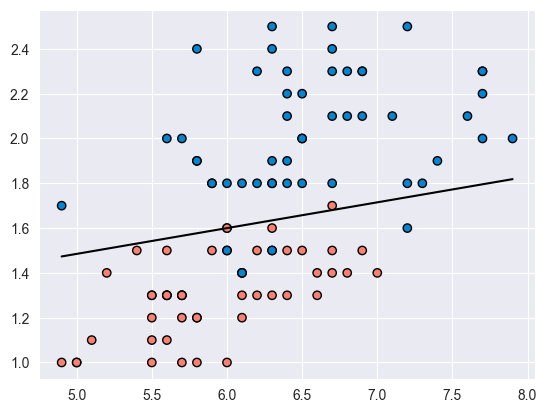
\includegraphics[height=0.35\textheight]{../../Images/HalfSp_2DIrisData.png}
\end{frame}

%%%%
\begin{frame}
    \frametitle{Logistic regression on the Iris data}
    Pictured below are selected lines found during the batch gradient descent. 
    
    \onslide<2->{
    As before, yellow-to-purple is progression through the procedure. Consecutive lines that are shown have $200$ updates between them; $\approx 4000$ updates in total.
    }

    \onslide<3->{
    The accuracy in this 2D projection is 92\% (the final hyperplane correctly labeled 92 out of 100).\footnote{Recall, the model labels the point with $+1$ when $f_{\omega}({\bf x}) \ge 0.5$.}
    }

    \onslide<4->{
    The model on the points in $\mathbb R^4$ took less updates (just under $3000$). It had 97\% accuracy on the data.
    }

    \vfill

    \centering
    \onslide<1->{
    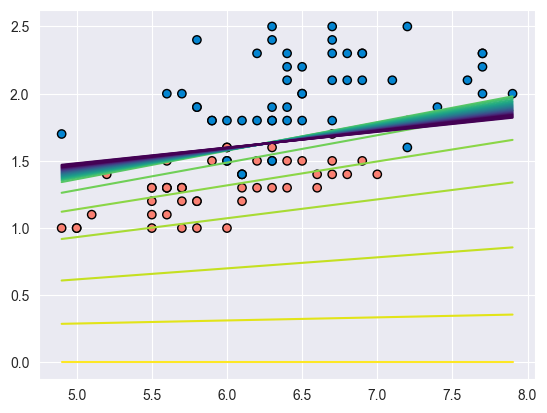
\includegraphics[height=0.35\textheight]{../../Images/GDon2DIrisData.png}
    }
\end{frame}

\end{document}